\documentclass[tikz,border=3.14mm]{standalone}
\usepackage{tikz}
\usetikzlibrary{arrows.meta, calc}

\begin{document}
	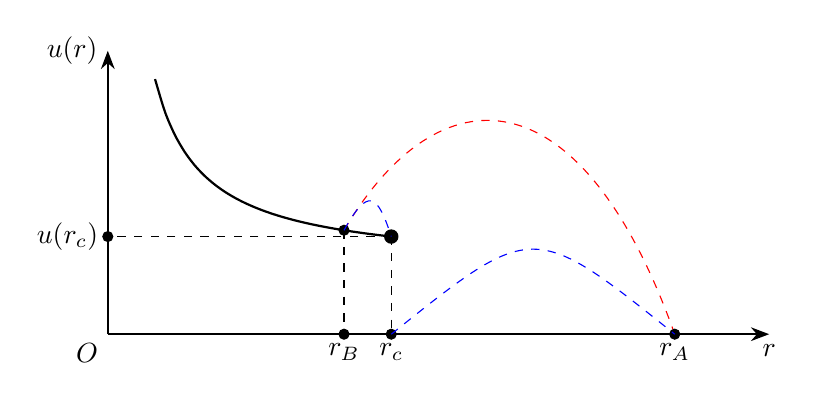
\begin{tikzpicture}[>=Stealth, scale=1.2]
		% 绘制坐标轴(无刻度,y轴适当长度)
		\draw[->, thick] (0,0) -- (7,0) node[below] {$r$}; % 延长x轴以适应新的抛物线范围
		\draw[->, thick] (0,0) -- (0,3) node[left] {$u(r)$};
		\node[below left] at (0,0) {$O$};
		
		% 绘制向上平移两倍的 1/x 曲线(在 x=3 处截断)
		\draw[domain=0.5:3, smooth, variable=\x, thick, black] 
		plot ({\x}, {1/\x + 0.7});
		
		% 在函数曲线x=3处截断
		\draw[fill=white, black] (3,1/3 + 0.7) circle (2pt);
		
		% 绘制垂直虚线(从函数曲线到x轴)
		\draw[dashed, black] (3,1/3 + 0.7) -- (3,0);
		\draw[fill=black] (3,0) circle (1.5pt) node[below] {$r_c$};
		
		% 绘制红色抛物线,从 x=2.5 到 x=6,顶点在中央 (4.25, y)
		% 使用贝塞尔曲线控制点调整抛物线形状和开口
		\draw[dashed, red] (2.5,1/2.5+0.7) 
		.. controls (3.5,2.8) and (5.0,2.8) .. (6,0); % 调整控制点使顶点在x=4.25附近,并保持开口向下
		
		% 抛物线左端点(与函数曲线相交)
		\draw[fill=black] (2.5,1/2.5+0.7) circle (1.5pt);
		% 从左交点向下做垂直虚线到x轴
		\draw[dashed, black] (2.5,1/2.5+0.7) -- (2.5,0);
		\draw[fill=black] (2.5,0) circle (1.5pt) node[below] {$r_B$}; 
		
		% 抛物线右端点(与x轴相交)
		\draw[fill=black] (6,0) circle (1.5pt) node[below] {$r_A$};
		
		% 为(3,1/3+0.7)点画一条横虚线到y轴,标记u(rc)
		\draw[dashed, black] (3,1/3 + 0.7) -- (0,1/3 + 0.7);
		\draw[fill=black] (0,1/3 + 0.7) circle (1.5pt) node[left] {$u(r_c)$};
		
		% ============ 新增的蓝色抛物线部分 ============
		% 1. 第一条蓝色抛物线:从 r_B 曲线上的点 (2.5, 1/2.5+0.7) 到 r_c 曲线上的点 (3, 1/3+0.7)
		% 顶点水平位置在 (2.5+3)/2 = 2.75,控制点用于形成开口向下的抛物线
		% 估算一个合适的顶点高度(低于两端点连线中点,且高度适中)
		\draw[dashed, blue] (2.5,1/2.5+0.7) 
		.. controls (2.75, 1.55) and (2.85, 1.5) .. (3,1/3+0.7); % 调整控制点使抛物线平滑且顶点在x=2.75附近
		
		% 2. 第二条蓝色抛物线:从 r_c 坐标轴上的点 (3, 0) 到 r_A 坐标轴上的点 (6, 0)
		% 顶点水平位置在 (3+6)/2 = 4.5,控制点用于形成开口向上的抛物线(从x轴向上凸)
		% 由于起点和终点都在x轴上,顶点高度需要为正才能形成向上的抛物线。选择一个适中的高度,例如y=1.2
		\draw[dashed, blue] (3,0) 
		.. controls (4.5,1.2) and (4.5,1.2) .. (6,0); % 控制点相同或非常接近以保持对称,顶点在x=4.5, y≈1.2
	\end{tikzpicture}
\end{document}